\chapter{Project Management}
\section{Agile Development Methodology}
To develop the wine quality classification, we decided to use Agile methodology. Agile methodology is an iterative approach to software development that emphasizes flexibility, collaboration, and rapid prototyping. We chose Agile methodology because it is well-suited to projects that require frequent feedback and adaptation to changing requirements.

\begin{figure}[H]
    \centering
    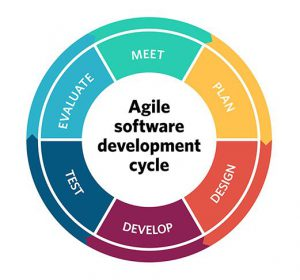
\includegraphics[scale = 0.9]{project_management/agile.jpg}
    \caption{Agile Development Methodology}
    \label{fig:Agile Development Methodology}
\end{figure}

\section{Trello}
We have used Trello's default agile board for task management. 
\begin{figure}[H]
    \centering
    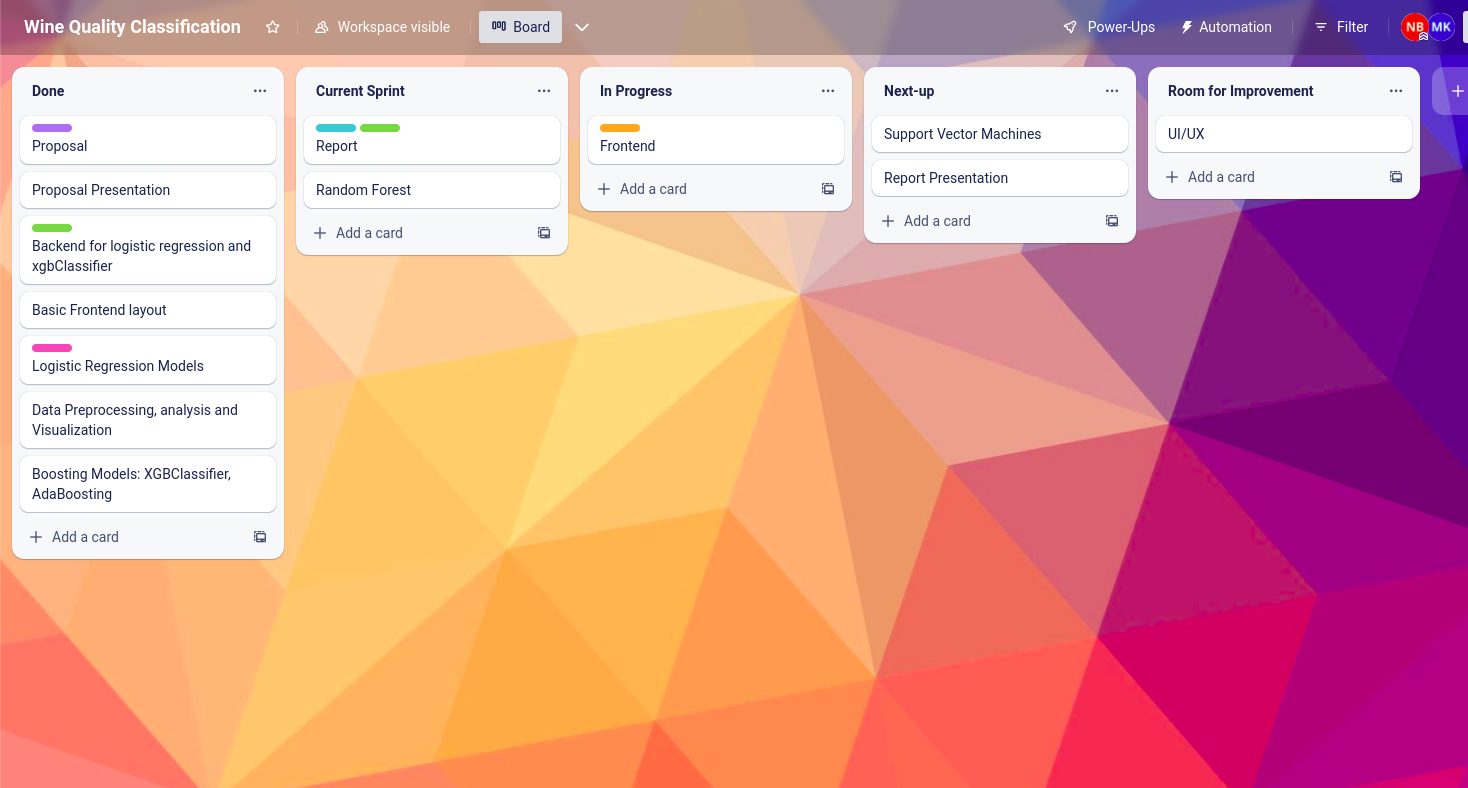
\includegraphics[scale = 0.33]{project_management/trello.png}
    \caption{Trello}
    \label{fig:Trello}
\end{figure}

\section{Discord}
We have used Discord server for effective communication and team meetings.

\begin{figure}[H]
    \centering
    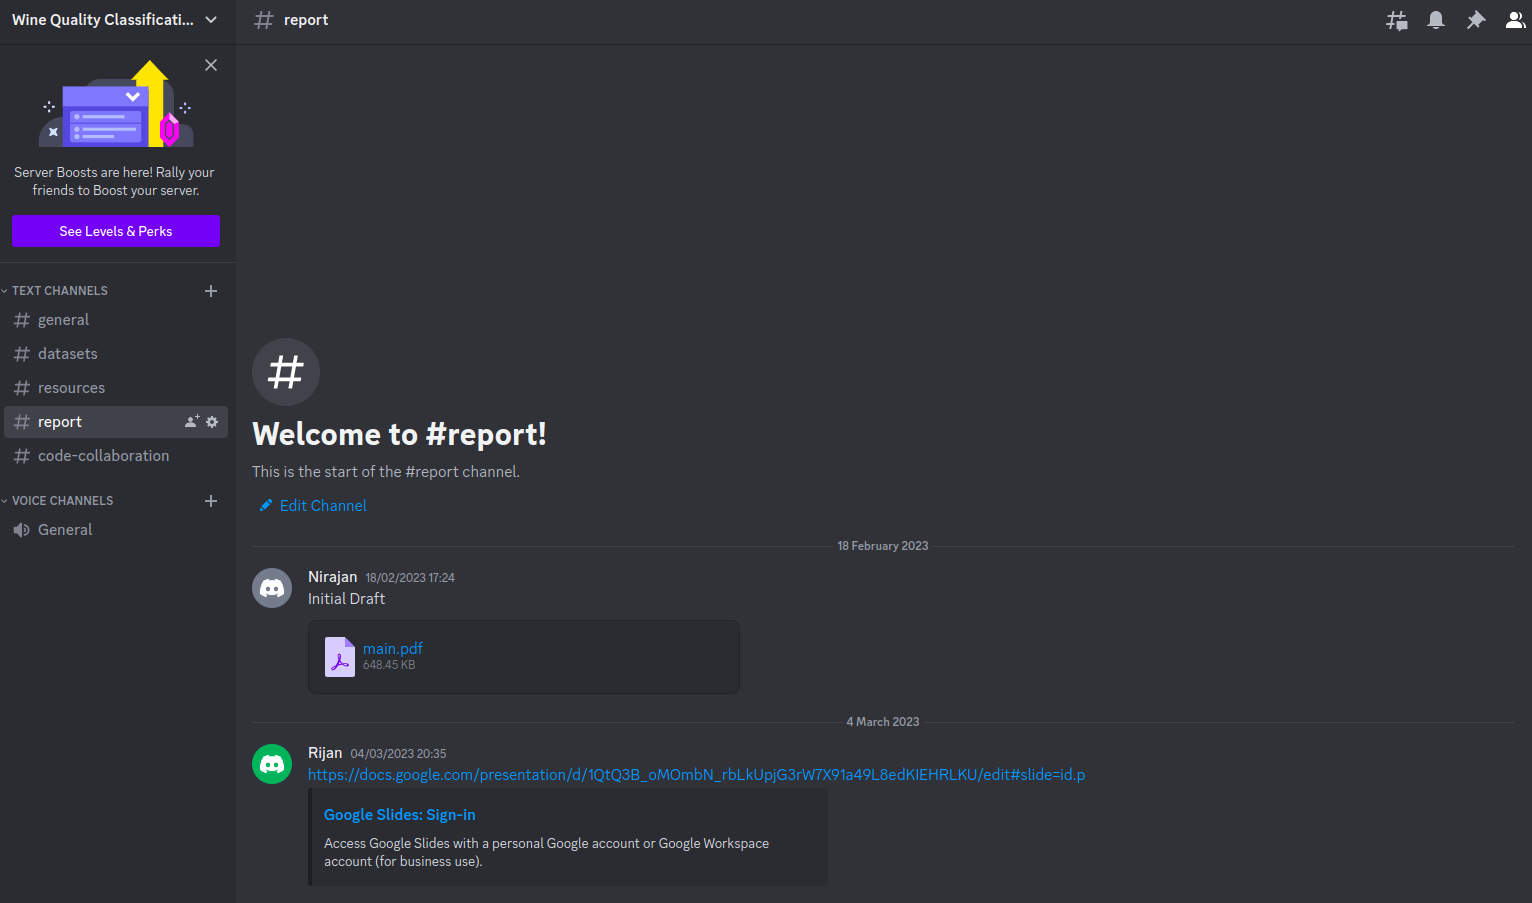
\includegraphics[scale = 0.3]{project_management/discord.png}
    \caption{Discord}
    \label{fig:Discord}
\end{figure}

\section{Excel}
We have used Excel for experiment tracking.
\begin{figure}[H]
    \centering
    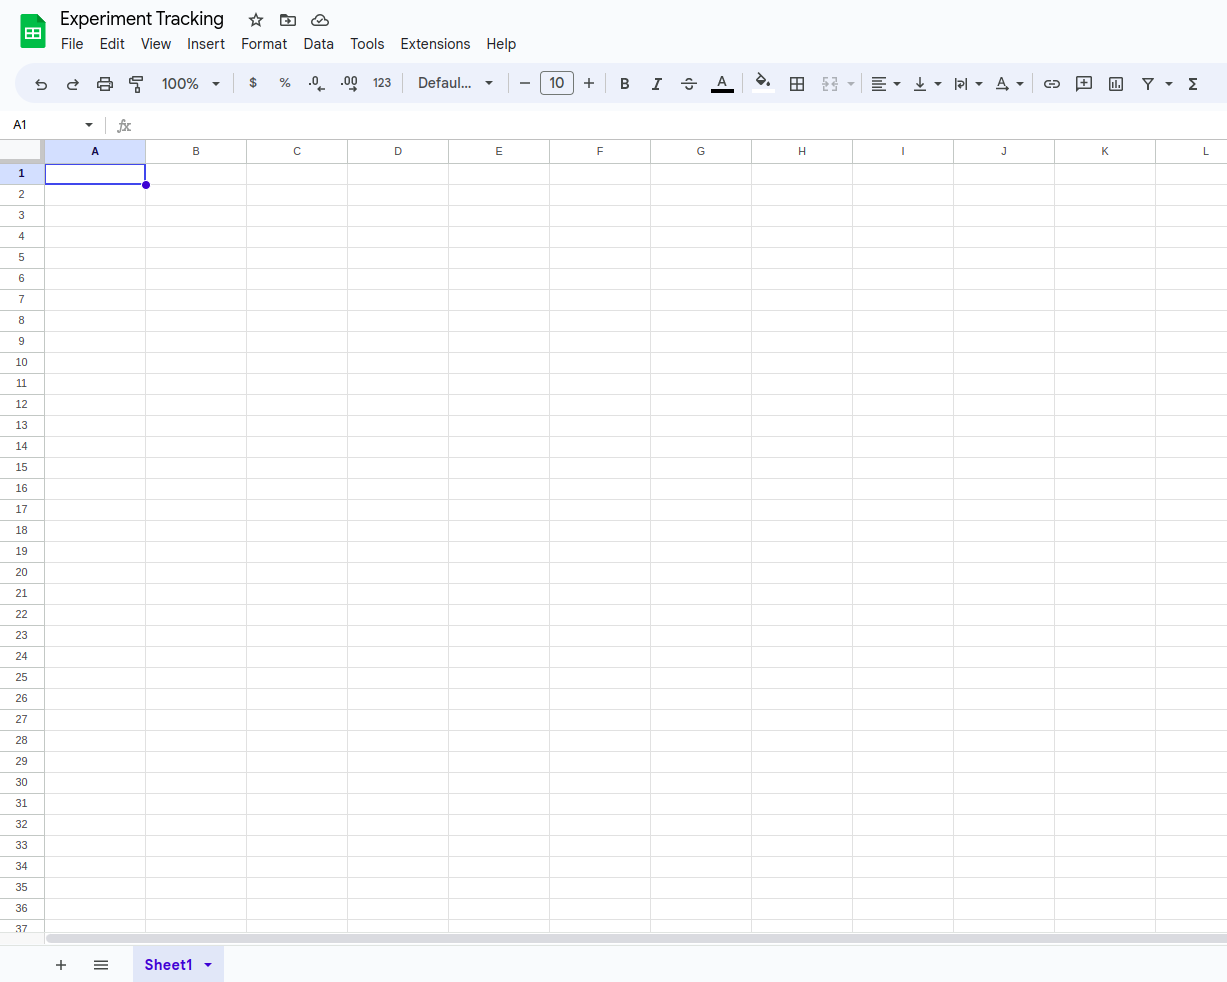
\includegraphics[scale = 0.39]{project_management/excel.png}
    \caption{Google Sheet}
    \label{fig:Google Sheet}
\end{figure}

